\documentclass[11pt,a4j]{jsarticle}

\usepackage{float,array,booktabs,here}
\usepackage{amsmath}
\usepackage[dvipdfmx]{graphicx}
\usepackage[top=20truemm,bottom=25truemm,left=20truemm,right=20truemm]{geometry}
\usepackage{url}

\makeatletter
\newcommand{\figcaption}[1]{\def\@captype{figure}\caption{#1}}
\newcommand{\tblcaption}[1]{\def\@captype{table}\caption{#1}}
\makeatother

\newcommand{\Maru}[1]{\ooalign{
\ifnum#1<10 \hfil\resizebox{.9\width}{.85\height}{#1}\hfil
\else
\hfil\resizebox{.6\width}{.8\height}{#1}\hfil
\fi
\crcr
\raise.1ex\hbox{$\bigcirc$}}}

%\usepackage[tableposition=top]{caption}



\begin{document}

% \title{フィルター}
% \author{hogehoge}
% \date{2015年5月9日}
% \maketitle


\section{目的}
射影行列の意味を理解し、それを用いて3次元形状を2次元に描画する。
また反対に多視点の画像から射影行列を推測し立体形状を復元する実験から
立体形状を得るために必要な理論を理解する


\section{理論}
\label{sec:理論}

\subsection{ディジタル画像}
\label{sub:ディジタル画像}
ピクセルは画像の要素を指す
ディジタル画像では、1つだけの最も小さい点のことであり、
画素は位置と色の二つのプロパティを持つ。 画素の位置の原点はいつも左方にあるが,
垂直方向は最初の画素に依存し位置の範囲は画質により決定される。
色は RGB 色空間が用いられ、Red、Green、Blueの3つの構成要素があり、
R、G、B それぞれの要素で 8bit ずつの情報を持つ。

\subsection{カメラについて}
\label{sub:カメラについて}

\subsection{射影行列}
\label{sub:射影行列}

\subsection{カメラキャリブレーション}
\label{sub:カメラキャリブレーション}

\subsection{ステレオ}
\label{sub:ステレオ}

\section{実験方法}
\label{sec:実験方法}

\subsection{サンプル画像への立方体の描写}
\label{sub:サンプル画像への立方体の描写}

\subsection{画像の射影行列の推測}
\label{sub:画像の射影行列の推測}

\subsection{多視点画像からの立体形状の復元}
\label{sub:多視点画像からの立体形状の復元}

\subsection{立体形状からアナグリフの作成}
\label{sub:立体形状からアナグリフの作成}

\section{結果}
\label{sec:結果}

\subsection{サンプル画像への立方体の描写}
\label{sub:result_box}

\begin{figure}[H]
  \centering
  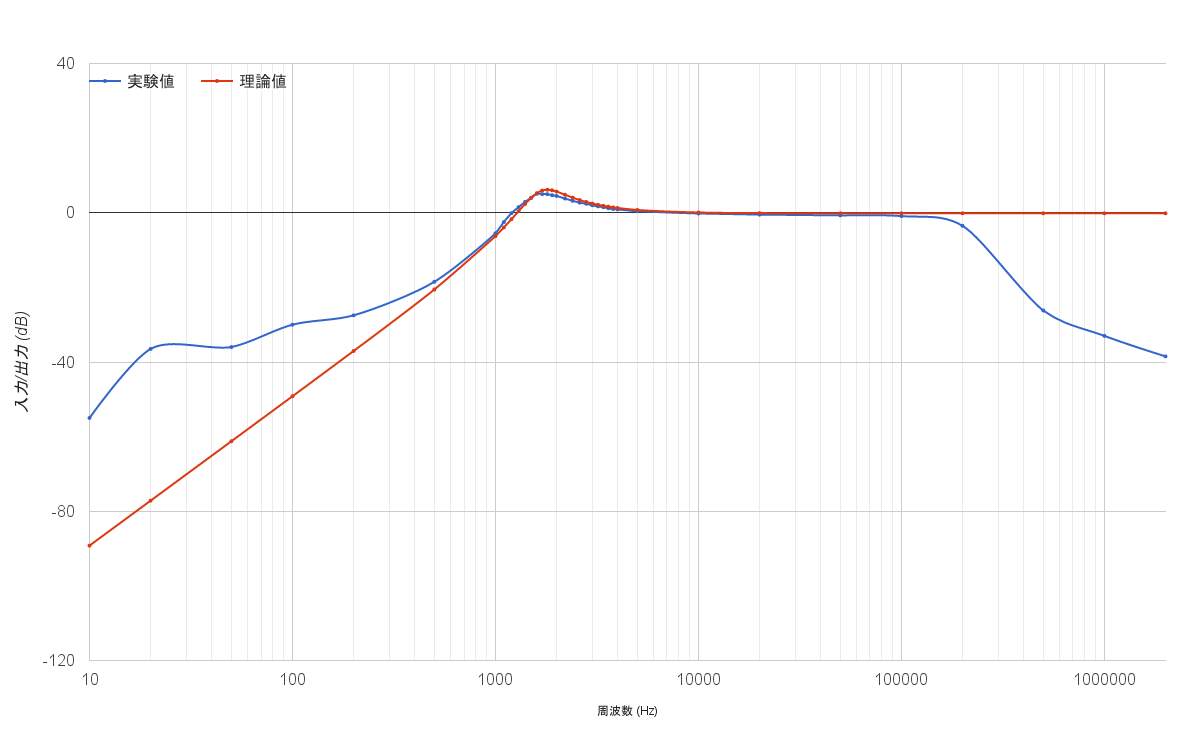
\includegraphics[height=100mm,bb=0 0 1188 735]{image/HPF.png}
  \figcaption{HPFの実験結果と理論値}
  \label{fig:hpf}
\end{figure}


\subsection{画像の射影行列の推測}
\label{sub:result_syaei}

\subsection{多視点画像からの立体形状の復元}
\label{sub:result_multimage}

\subsection{立体形状からアナグリフの作成}
\label{sub:result_anaglyph}

\section{考察}
\label{sec:考察}

\subsection{画像から推測した射影行列の誤差}
\label{sub:画像から推測した射影行列の誤差}



\subsection{オペアンプの理論特性}
\label{sub:オペアンプの理論特性}

演算増幅器のことをオペアンプという。
オペアンプの実際の端子と記号の関係は図\ref{fig:amp1},図\ref{fig:amp2}のように示すことができる。

\begin{table}[H]
	\begin{center}
	\begin{tabular}{cc}
	\begin{minipage}{0.49\hsize}
    \centering
    \includegraphics[scale=0.3]{image/opeamp1.ai} \\
    \figcaption{オペアンプの素子}
    \label{fig:amp1}
	\end{minipage} &
	\begin{minipage}{0.49\hsize}
		\centering
    \includegraphics[scale=0.3]{image/opeamp2.ai} \\
    \figcaption{オペアンプの中身}
    \label{fig:amp2}
	\end{minipage} \\
	\end{tabular}
	\end{center}
\end{table}

オペアンプの端子数はそれぞれに番号が付けられた8個であるが、通常使われるのは以下の5つの端子である。

$\Maru{2}$:逆相入力端子,
$\Maru{3}$:正相入力端子,
$\Maru{4}$:直流電源端子(-Vcc),
$\Maru{6}$:出力端子,
$\Maru{7}$:直流電源端子(+Vcc)


\subsection{加減算器}
\label{sub:加減算器}


加減算器は3入力信号の重み付け加減算を行う回路である。

\begin{table}[H]
	\begin{center}
	\begin{tabular}{cc}
	\begin{minipage}{0.49\hsize}
    \centering
    \includegraphics[scale=0.3]{image/addamp.ai} \\
      (a)回路
	\end{minipage} &
	\begin{minipage}{0.49\hsize}
		\centering
    \includegraphics[scale=0.3]{image/addamp_block.ai} \\
      (b)ブロック線図
	\end{minipage} \\
	\end{tabular}
	\end{center}
  \figcaption{加減算器}
  \label{fig:addamp}
\end{table}


図\ref{fig:addamp}のように入力信号を$\mathrm{v_1, v_2, v_3}$とした時,
\begin{align}
  v_0 &= k_3v_3 - k_2v_2 - k_1v_1 \\
  k_3 &= (1 + \frac{R_0}{R_1} + \frac{R_0}{R_2})(\frac{R_b}{R_a + R_b}) ,
  k_2 = \frac{R_0}{R_2} ,
  k_1 = \frac{R_0}{R_1}
\end{align}

このようになる。


\subsection{積分器}
\label{sub:積分器}

図\ref{fig:multamp}に積分器を示す。積分器は入力信号を連続時間で積分して出力する。

\begin{table}[H]
	\begin{center}
	\begin{tabular}{cc}
	\begin{minipage}{0.49\hsize}
    \centering
    \includegraphics[scale=0.3]{image/multamp.ai} \\
      (a)回路
	\end{minipage} &
	\begin{minipage}{0.49\hsize}
		\centering
    \includegraphics[scale=0.3]{image/mult_block.ai} \\
      (b)ブロック線図
	\end{minipage} \\
	\end{tabular}
	\end{center}
  \figcaption{積分器}
  \label{fig:multamp}
\end{table}

入力と出力の関係は複素数s = jωを用いて、
\begin{align}
  V_0(t) = \frac{-1}{RCs}V_1
\end{align}
となる。

\subsection{RCアクティブフィルタ}
\label{sub:RCアクティブフィルタ}

フィルタには低域通過フィルタ(LPF)、高域通過フィルタ(HPF)、帯域通過フィルタ(BPF)、帯域阻止フィルタ(BEF)がある。
LPFは入力に含まれる高い周波数成分のみが除去された出力信号となる。
同様に、HPFは低い周波数成分を、BPFはある一定の周波数成分以外を除去する。
今回の実験では抵抗とコンデンサ、演算増幅器を使ったRCアクティブフィルタを用いてLPF、HPF、BPFの2次伝達関数を実現する。

以下の図\ref{fig:filter}に実験で用いたRCアクティブフィルタの回路図とブロック線図を示した。

\begin{table}[H]
	\begin{center}
	\begin{tabular}{cc}
	\begin{minipage}{0.49\hsize}
    \centering
    \includegraphics[scale=0.4]{image/filter.ai} \\
      (a)回路
	\end{minipage} &
	\begin{minipage}{0.49\hsize}
		\centering
    \includegraphics[scale=0.4]{image/filter_block.ai} \\
      (b)ブロック線図
	\end{minipage} \\
	\end{tabular}
	\end{center}
  \figcaption{RCアクティブフィルタ}
  \label{fig:filter}
\end{table}


ここで、入力と出力の関係は図\ref{fig:filter}の(a)において$\Omega=\frac{1}{RC}$とおくと、以下の式が成り立つ。
\begin{align}
  \frac{V_L}{V_{in}} &= \frac{-K_2\Omega^2}{s^2 + K_1\Omega s + K_3\Omega^2} \,\,\,\,\,\, (LPF) \label{eq:filter1}\\
  \frac{V_B}{V_{in}} &= \frac{K_2\Omega s}{s^2 + K_1\Omega s + K_3\Omega^2} \,\,\,\,\,\, (LPF) \label{eq:filter2}\\
  \frac{V_H}{V_{in}} &= \frac{-K_2 s^2}{s^2 + K_1\Omega s + K_3\Omega^2} \,\,\,\,\,\, (LPF) \label{eq:filter3}
\end{align}


\section{結果}

\begin{table}[H]
  \caption{実験に用いたRCアクティブフィルタの素子の値}
  \label{tab:rc}
  \begin{center}
      \begin{tabular}{|c|c|c|c|}
        \hline
         & LPF & BPF & HPF \\ \hline
        $ R_{0}  (\mathrm{k\Omega}$) & \multicolumn{3}{c|}{9.85} \\ \hline
         & \multicolumn{3}{c|}{29.91} \\ \cline{2-4}
        \raisebox{0.8em}[1em]{R  ($\mathrm{\Omega}$)} & \multicolumn{3}{c|}{29.72} \\ \hline
        $ C  (\mathrm{pF}$) & \multicolumn{3}{c|}{1000} \\ \hline
        $ R_{1}  (\mathrm{k\Omega}$) & 100.0 & 63.2 & 10.02 \\ \hline
        $ R_{2}  (\mathrm{k\Omega}$) & \multicolumn{3}{c|}{99.9} \\ \hline
        $ R_{3}  (\mathrm{k\Omega}$) & 15.19 & 14.37 & 8.1 \\ \hline
        $ R_{4}  (\mathrm{k\Omega}$) & \multicolumn{3}{c|}{98.9} \\ \hline
        % & \multicolumn{2}{c|}{出力電圧/入力電圧 ($\mathrm{dB}$)} \\ \cline{2-3}
        % \raisebox{0.8em}[1em]{周波数($\mathrm{Hz}$)} & 測定値 & 理論値 \\ \hline

      \end{tabular}
  \end{center}
\end{table}



\begin{figure}[H]
  \centering
  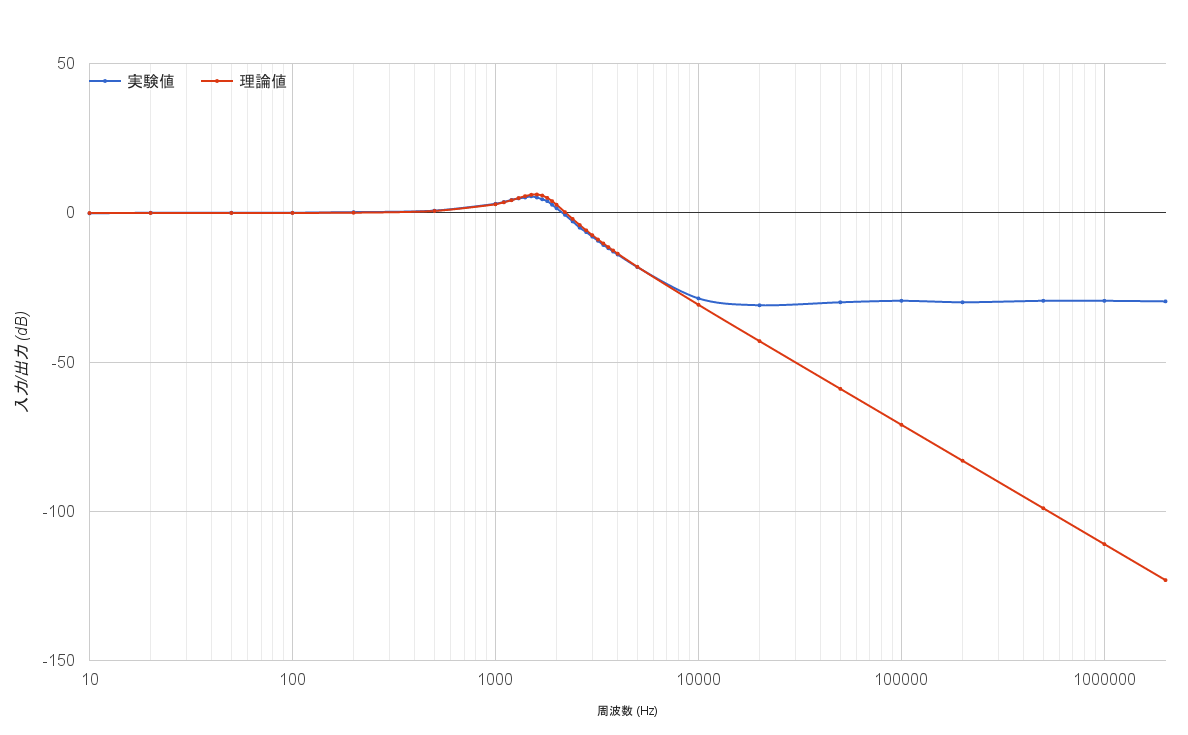
\includegraphics[height=100mm,bb=0 0 1188 735]{image/LPF.png}
  \figcaption{LPFの実験結果と理論値}
  \label{fig:lpf}
\end{figure}

\begin{figure}[H]
  \centering
  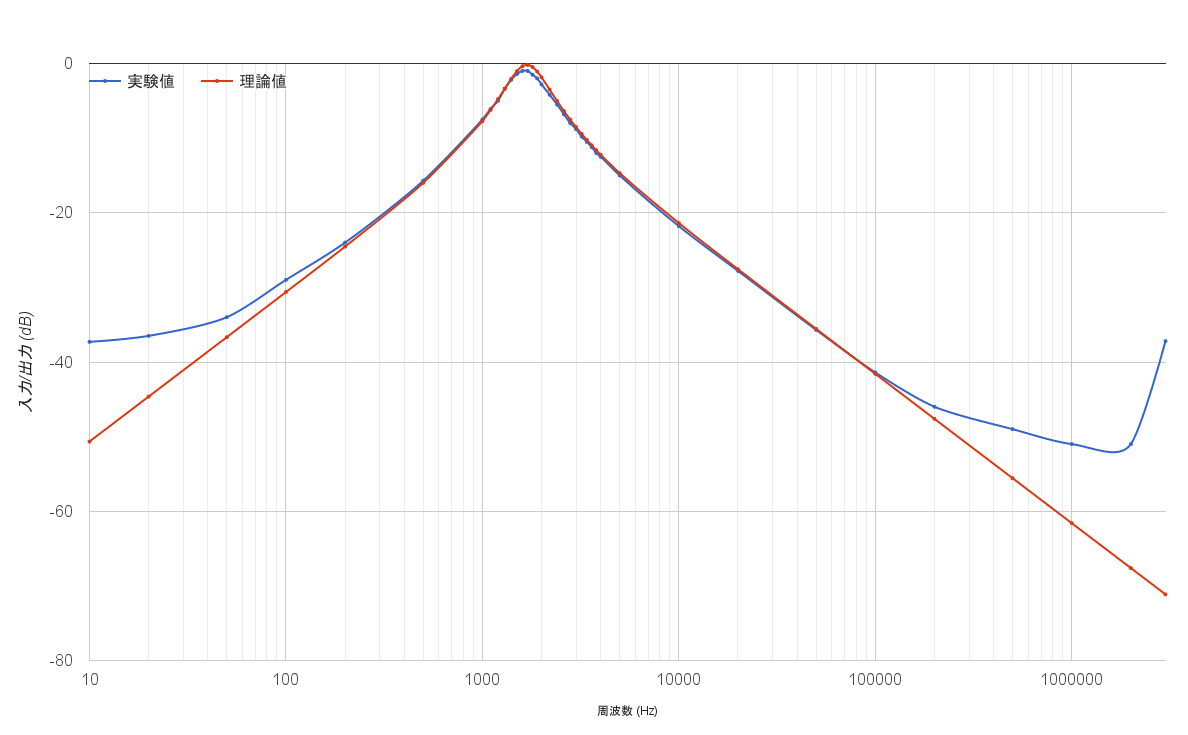
\includegraphics[height=100mm,bb=0 0 1188 735]{image/BPF.png}
  \figcaption{BPFの実験結果と理論値}
  \label{fig:bpf}
\end{figure}

\begin{figure}[H]
  \centering
  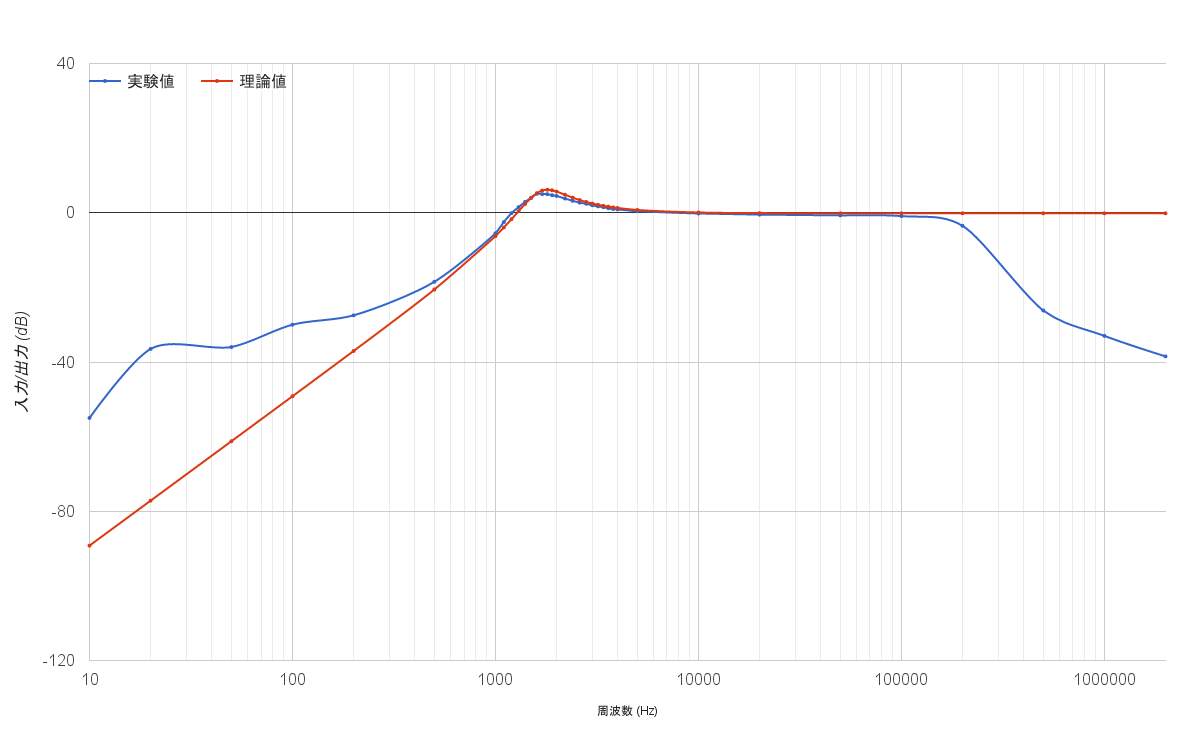
\includegraphics[height=100mm,bb=0 0 1188 735]{image/HPF.png}
  \figcaption{HPFの実験結果と理論値}
  \label{fig:hpf}
\end{figure}



\section{考察}
\label{sec:考察}

\subsection{理論値の導出方法}
\label{sub:理論値の導出方法}

式\ref{eq:filter1}、式\ref{eq:filter2}、式\ref{eq:filter3}に、$s=j\omega, \,\, \omega=2\pi f$
を代入して絶対値を取ると、以下の式のように表せる。

\begin{align}
  \left| \frac{V_L}{V_{in}} \right| &= \frac{K_2\Omega^2}{\sqrt{(K_3\Omega^2-\omega^2)^2 + (K_1\Omega\omega)^2}} \,\,\, (LPF) \\
  \left| \frac{V_B}{V_{in}} \right| &= \frac{K_2\Omega\omega}{\sqrt{(K_3\Omega^2-\omega^2)^2 + (K_1\Omega\omega)^2}} \,\,\, (BPF) \\
  \left| \frac{V_H}{V_{in}} \right| &= \frac{K_2\omega^2}{\sqrt{(K_3\Omega^2-\omega^2)^2 + (K_1\Omega\omega)^2}} \,\,\, (HPF) \\
\end{align}

表\ref{tab:rc}に示した実際の値をそれぞれ代入し、求めた値を$\mathrm{dB}$に変換するために、
$20log\left| \frac{V_L}{V_{in}} \right|$をとると理論値が求まる。

\subsection{積分器における周波数特性}
\label{sub:積分器における周波数特性}

\begin{itemize}
  \item 矩形波の入力をした時に三角葉を出力する理由 \\
   これは、積分器が入力信号を積分して出力するためである。また入力と出力は逆走であるので、矩形波が正の時に三角波の傾きは負となる。
  \item 周波数を下げていくと三角葉が大きくなる理由 \\
   周波数は$f=\frac{1}{T}$であるので、周波数を小さくするということは周期が長くなるということえある。
  それにより積分される時間が長くなるので、三角波の形が大きくなる。
  \item さらに周波数を下げると波形が歪む理由 \\
   これはオペアンプが電源電圧より大きな出力ができないためである。出力限界を超えた三角波は
  頂点が潰れ台形のような波形が出力され歪んだようになる。
\end{itemize}

\subsection{理論値と実験値のズレ}
\label{sub:理論値と実験値のズレ}

\begin{description}
  \item[オペアンプの理論特性とのズレ]\mbox{}\\
  実験から得られた 3 つのグラフを見ると、
  共通して周波数が極端に低いところと高いところで理論値からのずれが生じていることが読み取れる。
  この原因について考察する。

  周波数が0に近いところでのズレに関して、オペアンプへのオフセット値というものが関係していると考えられる。
  理想特性では出力電圧が極めて大きいため入力電圧は0と仮定してきたが、実際は0ではないことや、
  オペアンプの入力インピーダンスが極めて大きいため入力端子における電流が0と考えたが、
  これも実際は0ではなく電流が流れることよりずれが生じると考えられる。

  また、オペアンプは理想的に差動利得が無限大であると仮定しているが、
  実際のオペアンプでは周波数特性というものが存在する。
  実際には周波数が高くなるほど、その差動利得は小さくなり、周波数と差動利得の積は一定となる。
  これをゲインの積という。 実験値で高周波数域において理論値とずれたのはこれが一つの原因と考えられる。

  またスルーレートというパルス信号のように急激な変化を増幅する際に発生する増幅機能の限界を示す量がある。
  このスルーレートが追い付かなくなったことによるずれも考えられる。
  \item[自分なりの考察]\mbox{}\\
  実験書の3ページ目の逆相増幅器のブロック線図において$\mathrm{v_0 \, , \, v_1}$と書かれているが、
  ブロック線図はブロックの中に伝達関数で゙入出力を表すものであり、
  伝達関数はラプラス変換の比であるため、$\mathrm{V_0 \, , \, V_1}$と記すのが正しいであろうと思われる。
\end{description}

\section{感想}
\label{sec:感想}

今回実際にオペアンプをハンダなどを用いて実装し、LPF、BPF、HPFの動きをみたことでどちらの理解も深まった。
フィルタは他の授業でも学んでいたが、いまいぢ実感か湧かなかったが、゙実際に実験したことで、少し身近に感じることができた。



\begin{thebibliography}{9} %ケタ数(9:一桁、99:二桁)
\bibitem{saito} 斎藤英雄 , ``画像からの立体形状キャプチャ'' , 2016
\end{thebibliography}

\end{document}
